%%%%%%%%%%%%%%%%%%%%%%%%%%%%%%%%%%%%%%%%%
% Structured General Purpose Assignment
% LaTeX Template
%
% This template has been downloaded from:
% http://www.latextemplates.com
%
% Original author:
% Ted Pavlic (http://www.tedpavlic.com)
%
% Note:
% The \lipsum[#] commands throughout this template generate dummy text
% to fill the template out. These commands should all be removed when 
% writing assignment content.
%
%%%%%%%%%%%%%%%%%%%%%%%%%%%%%%%%%%%%%%%%%

%----------------------------------------------------------------------------------------
%	PACKAGES AND OTHER DOCUMENT CONFIGURATIONS
%----------------------------------------------------------------------------------------

\documentclass{article}

\usepackage{fancyhdr} % Required for custom headers
\usepackage{lastpage} % Required to determine the last page for the footer
\usepackage{extramarks} % Required for headers and footers
\usepackage{graphicx} % Required to insert images
\usepackage{lipsum} % Used for inserting dummy 'Lorem ipsum' text into the template
\usepackage{hyperref}

% Margins
\topmargin=-0.45in
\evensidemargin=0in
\oddsidemargin=0in
\textwidth=6.5in
\textheight=9.0in
\headsep=0.25in 

\linespread{1.1} % Line spacing

% Set up the header and footer
\pagestyle{fancy}
\chead{\hmwkClass\ - \hmwkClassInstructor\ - \hmwkTitle} % Top center header
\rhead{\firstxmark} % Top right header
\lfoot{\lastxmark} % Bottom left footer
\cfoot{} % Bottom center footer
\rfoot{Page\ \thepage\ of\ \pageref{LastPage}} % Bottom right footer
\renewcommand\headrulewidth{0.4pt} % Size of the header rule
\renewcommand\footrulewidth{0.4pt} % Size of the footer rule

\setlength\parindent{0pt} % Removes all indentation from paragraphs

%----------------------------------------------------------------------------------------
%	DOCUMENT STRUCTURE COMMANDS
%	Skip this unless you know what you're doing
%----------------------------------------------------------------------------------------

% Header and footer for when a page split occurs within a problem environment
\newcommand{\enterProblemHeader}[1]{
\nobreak\extramarks{#1}{#1 continued on next page\ldots}\nobreak
\nobreak\extramarks{#1 (continued)}{#1 continued on next page\ldots}\nobreak
}

% Header and footer for when a page split occurs between problem environments
\newcommand{\exitProblemHeader}[1]{
\nobreak\extramarks{#1 (continued)}{#1 continued on next page\ldots}\nobreak
\nobreak\extramarks{#1}{}\nobreak
}

\setcounter{secnumdepth}{0} % Removes default section numbers
\newcounter{homeworkProblemCounter} % Creates a counter to keep track of the number of problems

\newcommand{\homeworkProblemName}{}
\newenvironment{homeworkProblem}[1][Problem \arabic{homeworkProblemCounter}]{ % Makes a new environment called homeworkProblem which takes 1 argument (custom name) but the default is "Problem #"
\stepcounter{homeworkProblemCounter} % Increase counter for number of problems
\renewcommand{\homeworkProblemName}{#1} % Assign \homeworkProblemName the name of the problem
\section{\homeworkProblemName} % Make a section in the document with the custom problem count
\enterProblemHeader{\homeworkProblemName} % Header and footer within the environment
}{
\exitProblemHeader{\homeworkProblemName} % Header and footer after the environment
}

\newcommand{\problemAnswer}[1]{ % Defines the problem answer command with the content as the only argument
\noindent\framebox[\columnwidth][c]{\begin{minipage}{0.98\columnwidth}#1\end{minipage}} % Makes the box around the problem answer and puts the content inside
}

\newcommand{\homeworkSectionName}{}
\newenvironment{homeworkSection}[1]{ % New environment for sections within homework problems, takes 1 argument - the name of the section
\renewcommand{\homeworkSectionName}{#1} % Assign \homeworkSectionName to the name of the section from the environment argument
\subsection{\homeworkSectionName} % Make a subsection with the custom name of the subsection
\enterProblemHeader{\homeworkProblemName\ [\homeworkSectionName]} % Header and footer within the environment
}{
\enterProblemHeader{\homeworkProblemName} % Header and footer after the environment
}
   
%----------------------------------------------------------------------------------------
%	NAME AND CLASS SECTION
%----------------------------------------------------------------------------------------

\newcommand{\hmwkTitle}{Final Project} % Assignment title
\newcommand{\hmwkDueDate}{Tuesday,\ May\ 3,\ 2016} % Due date
\newcommand{\hmwkClass}{Big Data ILS - Z\ 604} % Course/class
\newcommand{\hmwkClassTime}{} % Class/lecture time
\newcommand{\hmwkClassInstructor}{Professor Liu} % Teacher/lecturer
\newcommand{\hmwkAuthorName}{asampath/jashjhav/nramanan/vpatani/sumbhand} % Your name

%----------------------------------------------------------------------------------------
%	TITLE PAGE
%----------------------------------------------------------------------------------------

\title{
\vspace{2in}
\textmd{\textbf{\hmwkClass:\ \hmwkTitle}}\\
\normalsize\vspace{0.1in}\small{Due\ on\ \hmwkDueDate}\\
\vspace{0.1in}\large{\textit{\hmwkClassInstructor\ \hmwkClassTime}}
\vspace{3in}
}

\author{\textbf{\hmwkAuthorName}}
\date{} % Insert date here if you want it to appear below your name

%----------------------------------------------------------------------------------------

\begin{document}

\maketitle

%----------------------------------------------------------------------------------------
%	TABLE OF CONTENTS
%----------------------------------------------------------------------------------------

%\setcounter{tocdepth}{1} % Uncomment this line if you don't want subsections listed in the ToC

\newpage
\tableofcontents
\newpage

%----------------------------------------------------------------------------------------
%	About The Problem
%----------------------------------------------------------------------------------------

% To have just one problem per page, simply put a \clearpage after each problem

\begin{homeworkProblem}[About the Problem]
\problemAnswer{ % Answer
\begin{center}
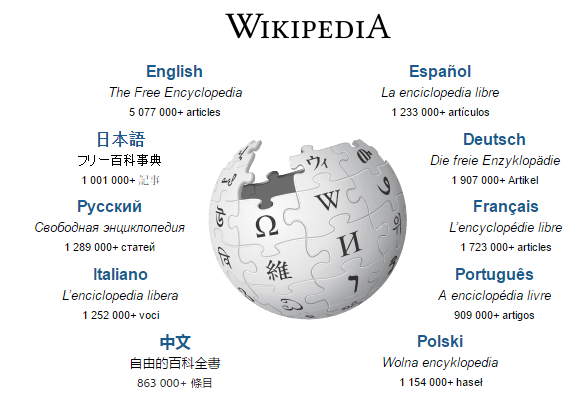
\includegraphics[width=0.75\columnwidth]{wiki}\\ % Example image
\end{center}
}
~\\~\\
The Question Answered here is a novel one. We are trying to predict the next edit of a certain page. Additionally we also predict whether if a page has their next edit within a certain time period or not. Interestingly enough. You wonder how could this serve as a business solution? Well, this definitely useful to Wikipedia to improve maintainability of their pages.\\~\\
How? They could assign more resources to a page having more edits and lesser to those which are infrequently edit. This helps them decide what to prioritize and how to make Wikipedia more and more efficient.\\~\\

\end{homeworkProblem}

%----------------------------------------------------------------------------------------
%	Dependencies
%----------------------------------------------------------------------------------------
\clearpage

\begin{homeworkProblem}[Dependencies] % Custom section title
We used an array of technologies during the course in order to achieve a superior model.
\begin{itemize}
\item Python
\item R Programming Language
\item MongoDB
\end{itemize}
~\\
Data Formats:
\begin{itemize}
\item XML
\item CSV
\item Pickle
\end{itemize}

\end{homeworkProblem}

%----------------------------------------------------------------------------------------
%	Files
%----------------------------------------------------------------------------------------
\clearpage
\begin{homeworkProblem}[Files]
\end{homeworkProblem}

%----------------------------------------------------------------------------------------
%	Raw Data
%----------------------------------------------------------------------------------------
\clearpage
\begin{homeworkProblem}[Raw Data] % Roman numerals
The original data set used for this problem statement is obtained from the \textbf{Wikimedia} dump service. We are using the revision data set dumped on 05-03-2016. The following attributes are available in the XML data set -
\begin{enumerate}
\item All metadata and data relating to wiki page is inside a ‘page’ tag.
\item Each page is referred to using a unique ‘id’ tag.
\item All metadata and data relating to revisions of a page are inside a ‘revision’ tag. A page can contain multiple revision tags.
\item Each revision has the following tags -
\begin{itemize}
\item An \textbf{id} tag to uniquely reference each revision
\item A \textbf{timestamp} tag to store the time and date of the revision
\item A \textbf{contributor} tag which stores details regarding the user who made the revision. It can contain the username or the IP address of the contributor. This tag may or may not be present.
\item A \textbf{text} tag stores the whole text of that page.
\item A \textbf{comment} tag which shows any comment for this wiki page. \\
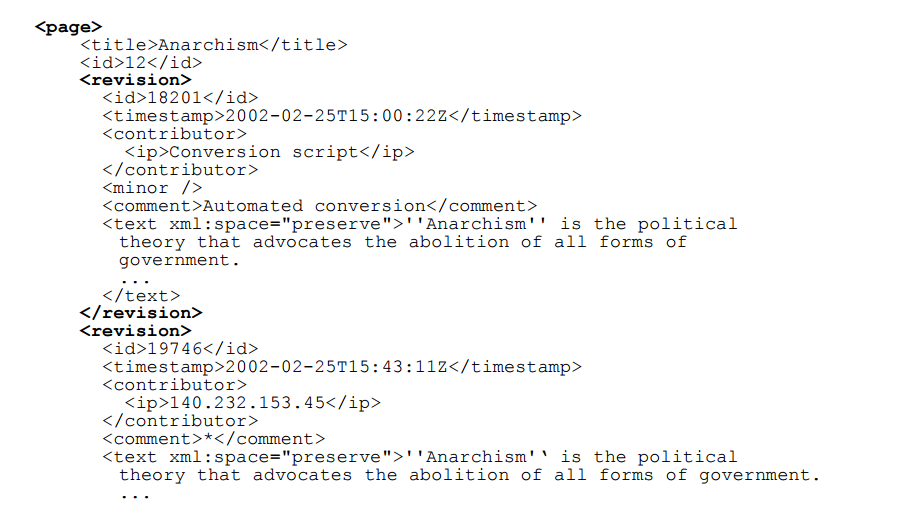
\includegraphics[width=0.75\columnwidth]{wikistruct}\\ % Example image

\end{itemize}

\end{enumerate}
\end{homeworkProblem}

%----------------------------------------------------------------------------------------
%	Indexing
%----------------------------------------------------------------------------------------
\clearpage
\begin{homeworkProblem}[Indexing]
We had begun Indexing the Wiki XML file with Mongo at the beginning, tried transforming it but failed at that attempt. The big problem here was primarily the data size and the unknown data structure. We could not open the file due to its extremely large size and hence we were unsure of the structure.

We had design our own indexing strategy. We are approaching the problem in the following steps:
\begin{itemize}
\item First we broke the XML file provided by Wikimedia into chunks so that we can make the file readable.
\item This was a major breakthrough since we finally realised the structure of the data.
\item We in our script are reading each line and looking for specific tags (Page ID \& 
Revision ID).
\item Our indexing Keys are a unique combination Page ID + Revision ID.\\
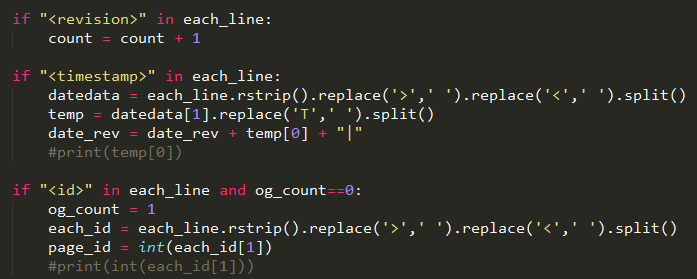
\includegraphics[width=0.75\columnwidth]{indexing}
\end{itemize}
\end{homeworkProblem}

%----------------------------------------------------------------------------------------
%	Feature Construction
%----------------------------------------------------------------------------------------
\clearpage
\begin{homeworkProblem}[Feature Construction]
Since the Xml data that we got is extremely large, to process the data we break this large XML into small chunks of XML. For every page in the XML,  we select certain features and write our feature for every page. Page id is the main index of our generated CSV. Using all of these edit dates for each page we generate more features for prediction of our model. The list of features added to the csv file -
\begin{itemize}
\item Page Id
\item Number of revisions
\item Date for the first revision of a page
\item Date for the last revision of a page
\item Year-wise count for number of revisions
\item Class Label
\end{itemize}
In approach1 and approach2 discussed below we give a detailed analysis of our newly generated features, the approach used to generate them, the need of these features and their influence on our accuracy.\\~\\
\end{homeworkProblem}

%----------------------------------------------------------------------------------------
%	Model Learning/Training
%----------------------------------------------------------------------------------------
\clearpage
\begin{homeworkProblem}[Model Learning/Training]
Our idea is to identify the editing pattern of individual pages in wikipedia. We took two approaches to evaluate our model and to see how it performs based on the provided training data.

\begin{homeworkSection}{Approach I}
We try to predict if a particular page would be edited in the next three months. We begin with targeting only those pages with multiple revisions. Timestamps(Date) is a key feature for our model. Every time a page is edited, we have a revision id and date for that revision.We use all of these edit dates in our model. Page id, revision count, previous edit date are some of the significant features we incorporate in this feature. We also generate another feature in this approach, called as a weighted revision factor. The way we do this is - we calculate the no of edits per page in every year since its creation. We give more weights to the edits that occurred post 2012 because the editing pattern is high in the recent years and this factor will greatly enhances our model prediction. Our accuracy increased by around 10-12 \% after adding this feature.\\ 
For evaluation, we test with by providing a choice of our date and we check for the all the pages if there would be an edit in the next 90 days from the provided date. We do this with a logistic regression and predict for the pages in our test data if they will be edited in next 90 days.\\
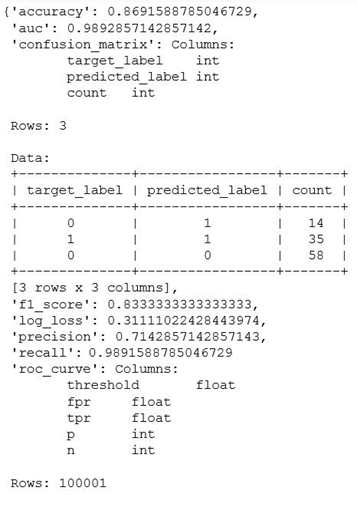
\includegraphics[width=0.75\columnwidth]{accuracy}
\end{homeworkSection}

\begin{homeworkSection}{Approach II}
In this approach, we try to predict the next edit date for a given page. This may sound similar to the previous approach but here we are trying to get the exact date of next date. This was a difficult task as only few pages in the data were frequently edited and predicting the next edit date without much previous edit data was challenging. We then tried to get the next edit month instead of the edit and this was relatively simple as the prediction scope was improved. Like in the previous approach, pageid, revision id revision count and edits are used as features here too. Some more important features for this approach are our last edit, second last edit date and average revision days.
\begin{itemize}
\item Last edit date is the date when a page was last edited.
\item Second last edit is that one edit before the latest revision. Last but one, in precise. 
\item Average revision days is a feature that we calculated for this approach. It is a ratio of the difference of days with respect to first and last edit date to the total number of revisions. This feature gives us as an idea about the frequency of the page being edited.
\end{itemize}~\\
With the available features and generated features we predict the month of our next edit. We keep the second last date as a reference and using the average revision days, next edit month is predicted. When we run this on test data, our predicted month and actual month of next edit are compared in our logistic model to evaluate the accuracy.\\
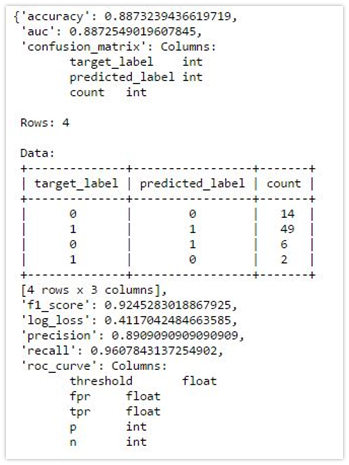
\includegraphics[width=0.75\columnwidth]{accuracy2}
\end{homeworkSection}

\begin{homeworkSection}{Additional Approach}
Random Forest uses an ensemble of decision trees to learn. An ensemble of classifiers has better classification performance than individual classifiers. Also an ensemble portrays better noise resilience. Here decision trees are built from a sample drawn from the training set. Not to forget these samples are with replacement. This prevents over fitting since it decreases the variance without changing the bias.\\
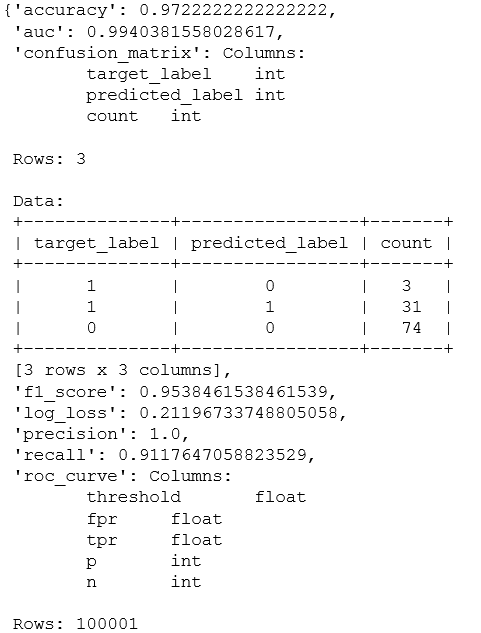
\includegraphics[width=0.75\columnwidth]{accuracy3}\\ % Example image
\end{homeworkSection}

\end{homeworkProblem}

%------------------------------------------------------------------------------------
%	Future Edit Learning Algorithm
%------------------------------------------------------------------------------------

\begin{homeworkProblem}[Future Edit Learning Algorithm]
The algorithm we wrote for learning future editing behaviour proceeds as follows:
\begin{itemize}
\item Parameter Selection: The main parameters of the learning algorithm are as follows:
\begin{enumerate}
\item Number of edits in certain time intervals prior to 8/4/2008  from the feature universe at each node for making an optimal splitting decision.
\item Number of Revisions is the Stopping condition on further node splitting. The lower this value, the more this, it under fits or over fits the data.
\item Weighted sum for edits in consecutive interval.
\begin{itemize}
\item Suppose page was edited ni times in the interval 2015-2016 which gets a weight of wi
And $n_i-1$ times in the interval 2015-2016 which gets a weight of $w_i-1$ , Given $w_i> w_i-1$
Weighted edits for each page would be\\
\[\sum_{i=0}^{k}W_i n_i/n_i\]
\end{itemize}
\item Most recent Edit Date
\item First existence of page
\item Text content difference between the first and the most recent version of it, gave very good performance.
\end{enumerate}

\item Splitting of Data:
\begin{itemize}
\item Sample Size: The sample size (less than or equal to the fully available sample size) used to train the model, 600 examples here In this case.
\item Test set: The number of examples to learn using the model, here it is 400 examples.
\end{itemize}

\item Logistic Regression
\begin{itemize}
\item 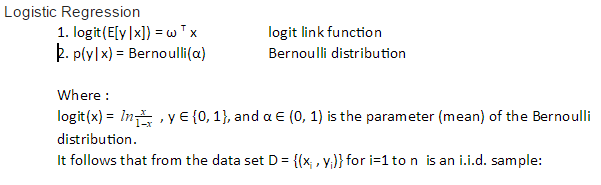
\includegraphics[width=0.75\columnwidth]{point3}\\ % Example image\\
\item 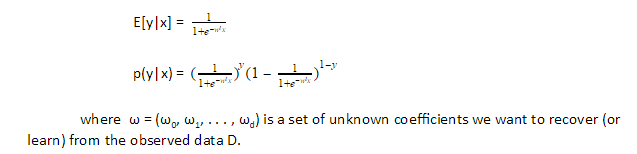
\includegraphics[width=0.75\columnwidth]{point3-1}\\ % Example image
\end{itemize}


\item We mention the Activation Function~\\
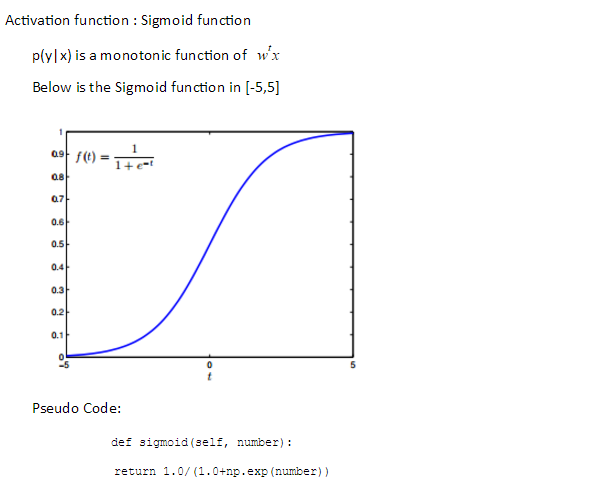
\includegraphics[width=0.75\columnwidth]{point4}\\ % Example image

\item Data Conclusion~\\
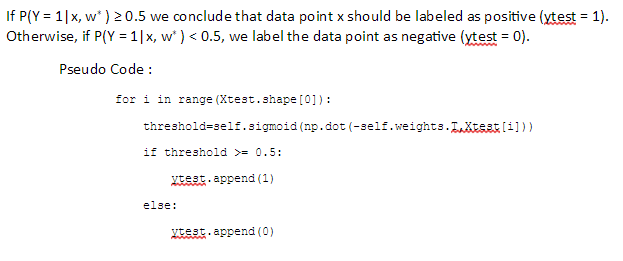
\includegraphics[width=0.75\columnwidth]{point5}\\ % Example image

\clearpage
\item Data Initial Weights~\\
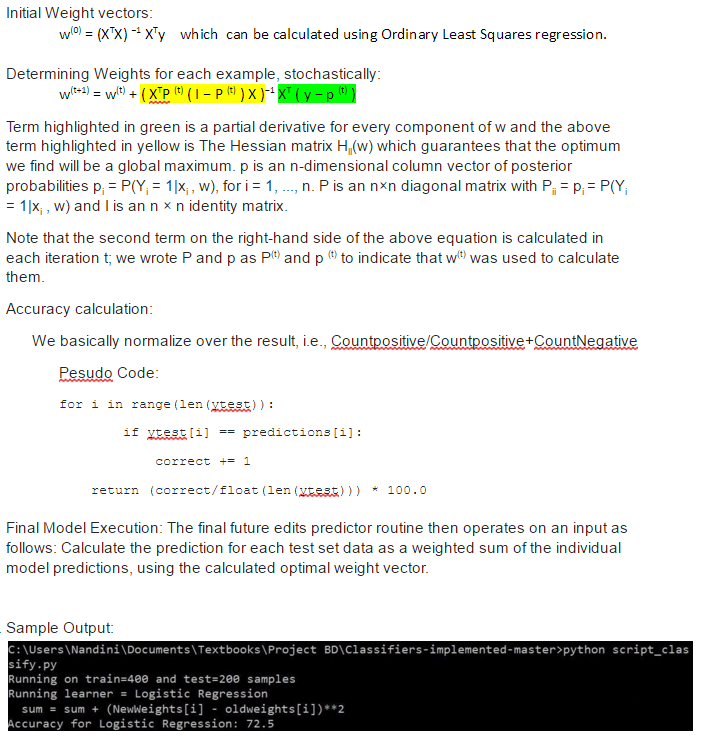
\includegraphics[width=0.75\columnwidth]{point6}\\ % Example image

\item We got an accuracy of close to 72.5 which isn't bad.
\end{itemize}

\end{homeworkProblem}

%----------------------------------------------------------------------------------------
%	Conclusions and Interpretation
%----------------------------------------------------------------------------------------
\clearpage
\begin{homeworkProblem}[Conclusions and Interpretation]
\begin{itemize}
The objective of this project is to quantitively understand what factors determine editing behavior. We hope to be able to answer questions, using these predictive models, why people stop editing or increase their pace of editing.
\end{itemize}
\end{homeworkProblem}

%----------------------------------------------------------------------------------------

\end{document}
